\documentclass[11pt,a4paper]{article}
\usepackage[margin=2.5cm]{geometry}
\usepackage{amsmath,amssymb,amsthm}
\usepackage{booktabs,array,multirow}
\usepackage{xcolor}
\usepackage{tcolorbox}
\tcbuselibrary{skins,breakable}
\usepackage{tikz}
\usetikzlibrary{arrows.meta,positioning,shapes.geometric,fit,backgrounds,calc,decorations.pathmorphing}
\usepackage{enumitem}
\usepackage{hyperref}
\usepackage[numbers,sort&compress]{natbib}
\bibliographystyle{unsrtnat}
\hypersetup{colorlinks=true,linkcolor=blue!60!black,urlcolor=blue!60!black,citecolor=green!50!black}

%─── Color palette ───────────────────────────────────────────────────────────
\definecolor{boxblue}{RGB}{220,235,255}
\definecolor{boxorange}{RGB}{255,240,210}
\definecolor{boxgreen}{RGB}{220,245,220}
\definecolor{boxtan}{RGB}{255,245,220}
\definecolor{boxpurple}{RGB}{240,225,255}
\definecolor{boxteal}{RGB}{210,240,238}
\definecolor{boxred}{RGB}{255,230,225}
\definecolor{rungorange}{RGB}{255,200,100}
\definecolor{rungblue}{RGB}{150,200,255}
\definecolor{runggreen}{RGB}{150,220,160}

%─── Macros ──────────────────────────────────────────────────────────────────
\newcommand{\term}[1]{\textbf{#1}}
\newcommand{\lean}[1]{\texttt{#1}}
\newcommand{\PHIMDL}{$\Phi_{\rm MDL}$}
\newcommand{\PhiMDL}{\Phi_{\rm MDL}}
\newcommand{\CMCA}{CMCA}
\newcommand{\ZS}{\mathbb{Z}_7}
\newcommand{\poly}{p}
\newcommand{\Mkink}{M_{\rm kink}}

%─── Theorem environments ────────────────────────────────────────────────────
\theoremstyle{definition}
\newtheorem{keyfact}{Key Fact}

%─── Title ───────────────────────────────────────────────────────────────────
\title{\textbf{The \boldmath$\Phi_{\rm MDL}$ Field:}\\[6pt]
\large From Discrete Certificate to Continuum Physics\\[8pt]
\normalsize
\href{https://novaspivack.com/research}{novaspivack.com/research}\quad
\href{https://doi.org/10.5281/zenodo.20560550}{P48 monograph (doi.org/10.5281/zenodo.20560550)}\\[4pt]\normalsize\textit{UGP Physics Tutorial Series}
\\[2pt]\small\href{https://doi.org/\TutorialDOI}{doi.org/\TutorialDOI}}
\author{Nova Spivack}
\newcommand{\TutorialDOI}{10.5281/zenodo.20657885}
\date{2026}

\begin{document}
\setcounter{tocdepth}{2}
\maketitle
\tableofcontents
\newpage

\begin{tcolorbox}[colback=blue!6,colframe=blue!40!black,
  title=\textbf{UGP Physics Tutorial Series}]
\textbf{Prerequisites (read first):} \href{https://doi.org/10.5281/zenodo.20657889}{\emph{The GTE Polynomial}} $\cdot$ \href{https://doi.org/10.5281/zenodo.20657919}{\emph{How the UWCA Works}} $\cdot$ \href{https://doi.org/10.5281/zenodo.20657906}{\emph{The Three-Tape CMCA}}\\[4pt]
\textbf{Next tutorials:} \href{https://doi.org/10.5281/zenodo.20657898}{\emph{How the Standard Model Quantum Numbers Emerge}} $\cdot$ \href{https://doi.org/10.5281/zenodo.20657870}{\emph{Gravity from Description-Length Minimization}}\\[4pt]
\textbf{See also:} \href{https://doi.org/10.5281/zenodo.20657861}{\emph{The Born Rule as a Theorem}}
\end{tcolorbox}

\begin{tcolorbox}[colback=boxgreen,colframe=green!50!black,
  title=\textbf{Claim-Strength Taxonomy}]
Throughout this tutorial, results are labeled with a confidence grade:
\begin{itemize}[itemsep=2pt]
  \item \textbf{$\mathbf{A}_{\rm Lean}$ (CatAL)} --- Machine-certified in Lean~4 with zero \texttt{sorry} and zero custom axioms.  Independently verifiable by anyone with Lean installed.
  \item \textbf{A/D (CatAD)} --- Analytically derived with full derivation, computationally confirmed.  Not yet machine-certified.
  \item \textbf{A (CatA)} --- Analytically derived; derivation complete but not independently machine-certified.
  \item \textbf{A/D (conditional)} --- Derived under a named, stated premise; the premise is itself an open problem or a CatB assumption.
  \item \textbf{B (CatB)} --- A stated working hypothesis or structural premise; not yet derived.
\end{itemize}
\end{tcolorbox}


%═════════════════════════════════════════════════════════════════════════════
\section{The Puzzle: From a 7-State Rule to Quantum Field Theory}
\label{sec:puzzle}
%═════════════════════════════════════════════════════════════════════════════

\begin{tcolorbox}[colback=boxblue,colframe=blue!40!black,title=The question this tutorial answers]
We have a single polynomial,
$p(L,C,R) = C + R - CR - LCR \pmod{7}$,
that updates a row of cells in seven possible states.
From this 19-bit rule, the masses of all elementary particles, the structure of
spacetime, and the laws of quantum mechanics can all be derived --- with zero free
parameters and over 300 machine-certified proofs.

\medskip
\noindent
\textbf{How?}  The cellular automaton is not the universe.
It is an algebraic certificate for a continuum quantum field,
$\PhiMDL$, which is what the universe is made of.
This tutorial explains what that distinction means and why it matters.
\end{tcolorbox}

\bigskip
\noindent
Imagine you receive a blueprint for a building.  The blueprint is a flat sheet of
paper covered in lines and dimensions.  The building is three-dimensional, made of
steel and glass, standing in a city.  The blueprint is not the building --- but it
contains everything you need to determine exactly what the building must be.

The GTE framework~\cite{SpivackGTECompleteFramework} works the same way:

\begin{itemize}
  \item The \term{blueprint} is the Chiral Minkowski Cellular Automaton (CMCA),
    described by the 19-bit polynomial $\poly$ over the Galois field GF(7).
    It is a finite, discrete algebraic object that can be machine-checked in a
    proof assistant (Lean 4).
  \item The \term{building} is $\PhiMDL$~\cite{SpivackPhiMDLField} --- a quantum field pervading all of
    $3{+}1$-dimensional Minkowski spacetime.
    It is the actual physical substance of the universe.
    Particles, forces, and spacetime itself emerge from its behavior.
\end{itemize}

The natural next question is: why do we need the blueprint at all?  Why not just work
directly with the building?  The answer is a technical one that turns out to be
profound: the discrete cellular automaton is the \emph{proof engine} for the continuum
field.  Algebraic facts that would be fiendishly difficult to prove directly in the
continuum become simple, finite, machine-checkable computations in the CA.
The CA certifies; the field realizes.

This tutorial is organized around three conceptual steps:
\begin{enumerate}
  \item Understanding the two-level architecture (§\ref{sec:twolevel}):
    the distinction between algebraic certificate (Level 1) and physical
    substrate (Level 2).
  \item The no-CA-replica theorem (§\ref{sec:noca}): why the universe
    \emph{cannot} be a cellular automaton at the substrate level, and what
    forces us to the continuum.
  \item The Algebraic Lifting Theorem (§\ref{sec:lifting}): the formal bridge
    that carries results from the certificate to the continuum field.
\end{enumerate}
The later sections then show what this machinery produces:
BPS kinks as particles (§\ref{sec:kinks}), the calibrated-reading picture of
the lattice spacing (§\ref{sec:reading}), and the three-rung ontological
ladder that organizes the whole framework (§\ref{sec:ladder}).

%═════════════════════════════════════════════════════════════════════════════
\section{The Two-Level Architecture: The Key Idea}
\label{sec:twolevel}
%═════════════════════════════════════════════════════════════════════════════

\subsection{Certificate and Substrate}

The most important conceptual distinction in the whole GTE framework is the following:

\begin{tcolorbox}[colback=boxorange,colframe=orange!60!black,title=The fundamental distinction]
\textbf{Level 1 (algebraic certificate):} The CMCA --- the discrete cellular
automaton with polynomial $\poly$ over GF(7).
This certifies \emph{what structures the universe must contain}, but is not
itself the physical universe.

\medskip
\noindent
\textbf{Level 2 (physical substrate):} $\PhiMDL$ --- the $\ZS$-symmetric
Klein-Gordon quantum field on $\mathbb{R}^{3+1}$.
This is what the universe actually is.  Particles, forces, and spacetime
geometry emerge from its dynamics.
\end{tcolorbox}

\bigskip
Three analogies illuminate why one can certify without being:

\begin{description}[leftmargin=1.5cm]
  \item[The blueprint analogy.]
    A building blueprint is a two-dimensional drawing that encodes everything about
    a three-dimensional building.  The blueprint is not the building --- you cannot
    live in it, and it is not made of glass --- but it certifies exactly what the
    building's structure must be.  The CMCA is the blueprint; $\PhiMDL$ is the building.

  \item[The program analogy.]
    A computer program (a text file of instructions) describes a computation, but
    it is not the computation itself.  The program can be machine-checked for
    correctness, stored cheaply, and transmitted instantly.  The running computation
    takes time, consumes energy, and unfolds in the physical world.  The CMCA is the
    program; $\PhiMDL$ is the running program-as-physical-process.

  \item[The thermometer analogy.]
    A thermometer does not contain the gas it measures --- it certifies a property
    (temperature) of that gas.  The gas is the physical substance; the thermometer
    reading is a certificate about the gas.  The CMCA certifies algebraic properties
    of $\PhiMDL$; those properties are then inherited by the continuum field.
\end{description}

\subsection{What the CMCA Certifies}

The CMCA can certify, in a completely rigorous, machine-checkable way, all of the
following \emph{algebraic} properties of the physical universe --- properties that hold
regardless of the spatial resolution or scale:

\begin{itemize}[itemsep=4pt]
  \item \textbf{Which particle types exist.}
    There are exactly five PSC-admissible winding sectors:
    $\{0, 2, 3, 4, 6\} \subset \ZS$,
    corresponding to the Standard Model particle classes.
    Machine-certified: \lean{psc\_admissible\_sectors} (zero sorry).

  \item \textbf{Why there are three generations.}
    The $\ZS^5$ orbit under $f_{\rm MDL}$ has exactly three non-vacuum orbit types,
    cycling with period 3.  This is a consequence of the $\ZS$ arithmetic, not a
    free input.  Machine-certified:
    \lean{three\_generations\_physical}, \lean{sm\_period3\_orbit\_chain} (zero sorry).

  \item \textbf{The electric charge formula.}
    $Q = w_{\rm c}/3$, where $w_{\rm c}$ is the centered representative of the
    $\ZS$ winding number.
    An electron has winding $w = 4$, so $Q = (4-7)/3 = -1$, exactly.
    Machine-certified: \lean{gte\_charge\_is\_linear\_projection} (zero sorry).

  \item \textbf{Particle statistics.}
    Sectors $\{2, 4, 6\}$ are non-primitive roots of $\ZS^*$ (order 3) and carry
    fermionic statistics.  Sector $\{3\}$ has order 6 and carries bosonic statistics.
    Machine-certified: \lean{gte\_winding\_identifies\_charged\_fermions} (zero sorry).

  \item \textbf{Charge quantization and colour confinement.}
    The $F_{21} = \ZS \rtimes \mathbb{Z}_3$ structure forces exact charge
    quantization and makes free coloured quarks MDL-forbidden.
    Machine-certified: \lean{gte\_charge\_is\_linear\_projection},
    \lean{psc\_forbids\_free\_colored\_quarks} (zero sorry).

  \item \textbf{The strong CP angle is zero.}
    Three independent algebraic proofs establish $\theta_{\rm QCD} = 0$ from
    $F_{21}$ group theory alone --- no axion required.
    Machine-certified (three independent theorems, zero sorry).
\end{itemize}

\begin{tcolorbox}[colback=boxteal,colframe=teal!50!black,title=What Level 1 cannot certify]
The CMCA cannot certify:
\begin{itemize}
  \item Exact Lorentz invariance (requires $M \to \infty$; see §\ref{sec:noca}).
  \item Particle masses (those come from the Level-2 orbit cascade and the field's
    energy, not from the CA's discrete rule).
  \item Specific CA patterns at the Compton scale that correspond to electrons
    or quarks (the exact microstructure is an open problem; the certificate
    certifies existence, not the specific glider pattern).
\end{itemize}
These properties require the continuum field $\PhiMDL$.
\end{tcolorbox}

\subsection{A Worked Example: The Electron at Both Levels}

To make the two-level picture concrete, trace the electron through both descriptions.

\medskip
\noindent\textbf{Level 1 (what the certificate says):}
The electron corresponds to the gen$_1$ beable configuration $[1,5,2,2,1]$ in
$\ZS^5$.
Its algebraic invariants are: winding $W_B = 4$, zero predecessors in the orbit
dynamics (``Garden of Eden'' --- it is the most algebraically stable),
and fermionic statistics (ord$(4) = 3$ in $\ZS^*$).
Charge: $Q = (4-7)/3 = -1$.
All machine-certified with zero sorry.

\medskip
\noindent\textbf{Level 2 (what the physical field says):}
The electron is a BPS topological kink in $\PhiMDL$ with winding $w = 4$,
connecting the fourth vacuum to the zeroth.
Its charge is $Q = -1$, its spin $J = 1/2$, and its mass $m_e = 0.511$\,MeV
from the Level-1 orbit cascade (the $N_{\rm eff} = 73$ seed value).

\medskip
\noindent\textbf{The formal chain:}
\begin{align*}
&\underbrace{[1,5,2,2,1],\; W_B{=}4,\;\text{Garden of Eden}}_{\text{Level-1 certificate}}\\
&\quad\xrightarrow{\lean{algebraic\_lifting\_theorem}\;(\text{zero sorry})}\\
&\underbrace{w{=}4 \text{ kink in }\PhiMDL,\;Q{=}-1,\;J{=}\tfrac{1}{2}}_{\text{Level-2 physical state}}
\;\xrightarrow{\text{orbit cascade}}\;
m_e = 0.511\text{ MeV}.
\end{align*}

Why is this remarkable?  We did not put in the charge, the statistics, or the mass
as free parameters.  They follow from the single 19-bit polynomial, via the
algebraic certificate, via the Lifting Theorem.

%═════════════════════════════════════════════════════════════════════════════
\section{The No-CA-Replica Theorem}
\label{sec:noca}
%═════════════════════════════════════════════════════════════════════════════

\subsection{The Question}

Many physicists and computer scientists have proposed that the universe \emph{is} a
cellular automaton --- that at the deepest level, spacetime consists of discrete
cells that update according to a local rule.
Wolfram's original ``new kind of science'' program, and 't Hooft's CA interpretation
of quantum mechanics, both take this view.

\medskip
The GTE framework takes a different position: the CA is the proof engine, not the
substrate.  But why?  What prevents the universe from simply being a CA?

\subsection{The Lorentz Invariance Argument}

The answer is Lorentz invariance --- the symmetry of special relativity that says
the laws of physics look the same to all observers moving at constant velocity.

Any finite cellular automaton has a finite lattice spacing.  With a finite lattice
spacing, there is a preferred frame: the frame in which the lattice is at rest.
At high velocities --- when the Lorentz factor $\gamma$ is large --- the lattice
structure becomes visible as small violations of Lorentz symmetry.

This violation can be quantified precisely.  For a CA with $M$ cells per unit
length, the \term{Nyquist residual} is:
\[
  \varepsilon_0(M) = \frac{\pi^2}{3M^2}.
\]
This measures the fractional error in the dispersion relation (how energy relates
to momentum) due to the discrete lattice.

\begin{center}
\begin{tabular}{@{}lcl@{}}
\toprule
\textbf{Model} & $\varepsilon_0(M) = \pi^2/(3M^2)$ & \textbf{Interpretation} \\
\midrule
CMCA at $M = 7$ & $6.71\%$ & CA scale error \\
$M = 100$ & $0.33\%$ & small but nonzero \\
$M = 10^6$ & $3.3 \times 10^{-12}$ & negligible but nonzero \\
$M \to \infty$ ($\PhiMDL$) & $0$ (exact) & exact Lorentz invariance \\
\bottomrule
\end{tabular}
\end{center}

\bigskip
\noindent
The key observation is: \emph{for any finite $M$, the error is strictly positive}.
There is no finite-resolution CA that achieves exact Lorentz invariance.
Only the continuum limit $M \to \infty$ achieves $\varepsilon_0 = 0$ exactly, and
that limit is $\PhiMDL$.

\begin{tcolorbox}[colback=boxred,colframe=red!50!black,
  title={Theorem: No-CA-Replica and $\PhiMDL$ Uniqueness (machine-certified)}]
For every finite lattice resolution $M > 0$:
\[
  \varepsilon_0(M) = \frac{\pi^2}{3M^2} > 0.
\]
No finite-resolution discrete model can exactly replicate $\PhiMDL$'s Lorentz
invariance.  The $M \to \infty$ continuum limit is the unique exact
Lorentz-invariant model in the $\ZS$ class, and that limit is $\PhiMDL$.

\smallskip\noindent
\textbf{Lean certifications:}\\
\lean{no\_finite\_ca\_exact\_lorentz\_replica} (zero sorry, ugp-lean) ---
$\varepsilon_0(M) > 0$ for all finite $M$.\\
\lean{phimdl\_is\_unique\_exact\_lorentz\_model} (zero sorry, ugp-lean) ---
$\PhiMDL$ is the unique zero-error model.\\
Both in \lean{CMCAContinuumLimit.lean}.
\end{tcolorbox}

\subsection{What the Theorem Does and Does Not Say}

A natural reaction: ``but the lattice error for $M = 7$ is only 6.71\%.  Why can't
we just use the CA and accept a 6.71\% error?''

Two responses:

\begin{enumerate}
  \item \textbf{Algebraic facts are M-independent.}
    All the algebraic structure certified by the CMCA --- charge quantization,
    three generations, $\theta_{\rm QCD} = 0$, etc.\ --- holds at every resolution
    $M \geq 1$.  The CA at $M = 7$ certifies these exactly, without any 6.71\%
    error.  What the error applies to is \emph{geometrical} properties: Lorentz
    boosts, dispersion relations, scattering amplitudes at high momentum.

  \item \textbf{Exact physics requires exact symmetry.}
    Quantum field theory and general relativity use exact Lorentz symmetry in
    essential ways.  Slightly broken Lorentz invariance is not a small perturbation
    --- it requires a fundamentally different theoretical framework.  The physical
    universe, as measured in experiments, shows no Lorentz violation down to scales
    of $10^{-32}$.  The unique object consistent with this is the continuum field
    $\PhiMDL$.
\end{enumerate}

\begin{tcolorbox}[colback=boxblue,colframe=blue!40!black,
  title={Important: the CMCA is not ``wrong'' --- it is \emph{not the substrate}}]
The no-CA-replica theorem does not mean the CMCA is a bad or incorrect model.
It means the CMCA is the wrong \emph{kind} of object to be the physical substrate.
The CMCA is a certificate, not a substrate.
A blueprint is not wrong --- it's just not a building.
\end{tcolorbox}

\subsection{Contrast with Other CA Proposals}

This is where GTE differs most sharply from other CA-based physics programmes:

\medskip
\begin{center}
\begin{tabular}{@{}lcc@{}}
\toprule
\textbf{Framework} & \textbf{CA status} & \textbf{Resolves Lorentz problem?} \\
\midrule
Wolfram (original) & CA \emph{is} the universe & No (preferred frame remains) \\
't Hooft CA interpretation & CA \emph{is} the substrate & No (approximate) \\
\textbf{GTE} & CA is the \emph{certificate} & Yes (continuum limit is exact) \\
\bottomrule
\end{tabular}
\end{center}

\medskip\noindent
The GTE resolution: keep the CA as a proof engine (it is invaluable for
certifying algebraic facts), but identify the physical substrate with the
continuum field whose algebraic structure the CA certifies.
The no-CA-replica theorem is what forces this identification --- and the Algebraic
Lifting Theorem (§\ref{sec:lifting}) is the bridge that makes it work.

%═════════════════════════════════════════════════════════════════════════════
\section{The Algebraic Lifting Theorem}
\label{sec:lifting}
%═════════════════════════════════════════════════════════════════════════════

\subsection{What ``Lifting'' Means}

The Lifting Theorem is the formal statement that results proved in the CA
have corresponding statements in the continuum field.

A useful analogy from mathematics: model-theoretic completeness.
In logic, a theory $T$ is complete if every statement that is true in the
intended model is provable from the axioms.
The Lifting Theorem plays a similar role: every algebraic fact proved in the
CMCA (the discrete model) is true in $\PhiMDL$ (the intended physical realization).
The CA is the model; $\PhiMDL$ is the full theory.

More concretely: suppose you prove in the CA that winding number is conserved
at every interaction vertex.  The Lifting Theorem guarantees that winding number
is also conserved at every interaction vertex in $\PhiMDL$, at the Compton scale.

\begin{tcolorbox}[colback=boxgreen,colframe=green!50!black,
  title={Theorem: Algebraic Lifting (machine-certified, zero sorry, zero custom axioms)}]
Let $B$ be a PSC-admissible beable (a configuration in the CMCA orbit) with
positive dynamical weight.
Then $B$ determines a physical observable at the Compton scale carrying the same
$\ZS$ winding number, $\mathbb{Z}_3$ color charge, and generation index as $B$.

In particular: charge quantization, color structure, the three-generation
hierarchy, and $S$-matrix quantum numbers proved at the beable level hold at the
physically observable Compton scale.

\smallskip\noindent
\textbf{Lean cert:} \lean{algebraic\_lifting\_theorem}
(\lean{LiftingTheorem.lean}, ugp-lean, zero sorry, zero custom axioms).
\end{tcolorbox}

\subsection{The Complementary Direction: Algebraic Descent}

The Lifting Theorem has a complementary direction that goes from the
continuum back to the discrete:

\begin{tcolorbox}[colback=boxblue,colframe=blue!40!black,
  title={Theorem: Algebraic Descent (machine-certified, zero sorry)}]
Every $F_{21} = \ZS \rtimes \mathbb{Z}_3$ conservation law, charge quantization
condition, and generation structure certified at the discrete CMCA level holds in
any continuum realization at any lattice resolution $M \geq 1$.

Charge quantization, color confinement, asymptotic freedom, and the strong-CP
resolution $\theta_{\rm QCD} = 0$ are $M$-independent.
Only geometric properties (Lorentz invariance, scattering amplitudes) require
$M \to \infty$.

\smallskip\noindent
\textbf{Lean cert:} \lean{algebraic\_descent\_theorem}
(\lean{AlgebraicDescentTheorem.lean}, ugp-lean, zero sorry).
\end{tcolorbox}

\subsection{What the Two Theorems Mean Together}

\begin{tcolorbox}[colback=boxtan,colframe=orange!50!black,title=The bidirectional bridge]
\textbf{Lifting} says: if you prove it in the CA, it exists in the field.

\textbf{Descent} says: whatever the field must respect, the CA also enforces.

Together: the CMCA and $\PhiMDL$ are \emph{algebraically equivalent in the SM
winding sector} --- two descriptions of the same object at different scales.
Neither level can produce anything the other forbids.

\smallskip
Practical consequence: proving a theorem about a simple cellular automaton
is proving a theorem about particle physics, provided the theorem concerns
the $F_{21}$ winding sector (which governs SM quantum numbers, interaction
vertices, and generation structure).
\end{tcolorbox}

\subsection{A Plain-English Example}

Consider the statement: ``An isolated quark cannot be observed as a free particle.''

\medskip
\noindent
\textbf{In the CA (Level 1):}
A free quark would carry winding $w \in \{2, 6\}$ (for up or down quarks).
Displaying such a state costs $\log_2(9) \approx 3.17$ extra MDL bits to specify
which color it carries.  MDL minimality forbids this: isolated colored states
are PSC-inadmissible.
Machine-certified: \mbox{\lean{psc\_forbids\_free\_colored\_quarks}} (zero sorry).

\medskip
{\sloppy
\noindent
\textbf{By Descent to the field ($\PhiMDL$):}
The Descent Theorem guarantees that the PSC-inadmissibility established at
Level~1 holds at every resolution $M \geq 1$, including the continuum.
Therefore, $\PhiMDL$ also forbids free colored quarks: color confinement is
an exact algebraic fact of the continuum theory, certified by the CA.
\par}

\medskip\noindent
This is the mechanism by which a 19-bit polynomial over a 7-element finite
field certifies --- with zero sorry and zero free parameters --- that
quark confinement holds in the physical universe.

%═════════════════════════════════════════════════════════════════════════════
\section{BPS Kinks: The Physical Particles}
\label{sec:kinks}
%═════════════════════════════════════════════════════════════════════════════

\subsection{What a Kink Is}

A \term{kink} in a field theory is a stable topological excitation --- a region
where the field permanently transitions from one vacuum state to another.

The $\PhiMDL$ field has a $\ZS$-symmetric potential:
\[
  V(\Phi) = \frac{m_\varphi^2}{49}\bigl(1 - \cos 7\Phi\bigr).
\]
This potential has seven degenerate minima (``vacua'') at
$\Phi_k = 2\pi k/7$ for $k \in \{0,1,\ldots,6\}$, equally spaced around the
unit circle in field space.
Think of seven evenly-spaced valleys arranged in a ring; the field can sit
in any of them with zero energy cost.

A kink is a field configuration that starts in one valley as $x \to -\infty$
and ends in a different valley as $x \to +\infty$.  The transition region ---
the smooth interpolation between two vacua --- is the kink.

\begin{tcolorbox}[colback=boxgreen,colframe=green!50!black,title=Particles as topology]
A particle is not a tiny ball of stuff occupying a small region.
It is a topological feature of the $\PhiMDL$ field: a permanent winding of
the field from one vacuum to another.

What we call ``an electron'' is a kink in the $\PhiMDL$ field with
winding number $w = 4$, connecting the fourth vacuum to the zeroth.
The winding number is the particle's identity card.
\end{tcolorbox}

\subsection{The Rope Analogy}

Here is a helpful picture.  Imagine a very long rope that can take on seven
colors, equally spaced on a color wheel.  In empty space, the rope is uniform
(say, color 0 --- the vacuum state).  A particle corresponds to a region where
the rope permanently changes color --- say, from color 0 to color 4 over a
short stretch.  To the left, the rope is color 0; to the right, it is color 4.
That color-change region is the kink.

To destroy the particle, you need a region where the rope returns from color 4
to color 0 --- that is its antiparticle.  When the particle and antiparticle
meet and annihilate, the rope returns to uniform color 0 everywhere.

The ``colors'' here are the $\ZS$ winding number values.  Two color-steps
gives an up quark; three color-steps gives a $W^+$ boson; four color-steps
gives an electron.  There is no ``substance'' here --- the particle is a
configuration, not a material.

\subsection{Why BPS Kinks Are Special: Stability and the Energy Bound}

Not every kink is a physical particle.  The physically relevant kinks are
\term{BPS-saturated} (Bogomolny-Prasad-Sommerfield): they satisfy the first-order
equation
\[
  \frac{d\Phi}{dx} = \sqrt{2V(\Phi)},
\]
which guarantees that the kink has the \emph{minimum possible energy} for its
topological class.  This means:
\begin{itemize}
  \item The kink is exactly stable: any small deformation increases its energy.
  \item The kink has zero longitudinal stress ($T_{11} = 0$): it has
    ``no internal pressure'' and propagates without distortion.
  \item The kink mass is a clean, universal formula: $\Mkink = (8/49)\,m_\varphi$.
\end{itemize}

With $m_\varphi = m_\tau = 1776.86$\,MeV (the tau mass, derived from the
Self-Consistency Condition, not a free input):
\[
  \Mkink = \frac{8}{49} \times 1776.86\text{ MeV} = 290.10\text{ MeV}.
\]
This is the hadronic energy scale --- the scale at which the strong interaction
operates.  Machine-certified: \lean{mkink\_from\_scc} (zero sorry, ugp-lean).

\subsection{The SM Particle Assignment Table}

The $\ZS$ potential has seven vacua and six non-trivial kink sectors
($w \in \{1,2,3,4,5,6\}$).  Not all six are physically admissible.
The PSC-admissibility condition (from the dark-mirror structure of
$F_{21} = \ZS \rtimes \mathbb{Z}_3$) restricts to five sectors,
eliminating $\{1,5\}$.
The five surviving sectors map exactly to the SM particle classes:

\begin{center}
\begin{tabular}{@{}cclcc@{}}
\toprule
\textbf{Winding $w$} & \textbf{Charge $Q = w_{\rm c}/3$}
  & \textbf{Particle type} & \textbf{Statistics} & \textbf{Cert} \\
\midrule
$0$ & $0$ & Vacuum / photon / neutrino & bosonic & zero sorry \\
$2$ & $+2/3$ & Up-type quarks ($u,c,t$) & fermionic & zero sorry \\
$3$ & $+1$ & $W^+$ boson / positron & bosonic & zero sorry \\
$4$ & $-1$ & Charged leptons ($e^-,\mu^-,\tau^-$), $W^-$ & fermionic & zero sorry \\
$6$ & $-1/3$ & Down-type quarks ($d,s,b$) & fermionic & zero sorry \\
\bottomrule
\end{tabular}
\end{center}

The charge formula uses the centered representative $w_{\rm c} = w$ for $w \leq 3$
and $w_{\rm c} = w - 7$ for $w \geq 4$.
So $w = 4$ gives $Q = (4-7)/3 = -1$ (electron) and
$w = 6$ gives $Q = (6-7)/3 = -1/3$ (down quark).
All assignments follow algebraically from $p$; no assignment rule is needed.

\subsection{Three Generations from One Field}

The three Standard Model generations do not require three separate fields.
They arise from the three non-vacuum orbit types of the $\ZS^5$ ring under
$f_{\rm MDL}$: gen$_1 \to$ gen$_2 \to$ gen$_3 \to$ gen$_1$, cycling with period~3.

The first generation ($e^-$, $u$, $d$, $\nu$) corresponds to the Garden of Eden
orbit type: it has \emph{no predecessors} under the orbit dynamics, making it
algebraically the most stable --- and the lightest.
In the SRRG orbit cascade, this Garden-of-Eden status corresponds to the Lepton
Seed value $N_{\rm eff} = 73$ (the arithmetic origin of the cascade), the smallest
of the three lepton addresses; since kink mass scales with $N_{\rm eff}$, the GoE
generation carries the minimum mass.
Machine-certified:
\lean{fmdl\_gen1\_is\_garden\_of\_eden}, \lean{three\_generations\_physical} (zero sorry).

\begin{tcolorbox}[colback=boxpurple,colframe=purple!50!black,
  title=Topological protection: why particles are stable]
A kink cannot spontaneously unwind.  To transition from $w=4$ (electron) to
$w=0$ (vacuum) requires the field to cross an infinite energy barrier
(in the continuum limit $M\to\infty$).  Particle stability is not protected
by a symmetry imposed by hand --- it is a geometric consequence of topology.
\end{tcolorbox}

%═════════════════════════════════════════════════════════════════════════════
\section{The Calibrated-Reading Resolution}
\label{sec:reading}
%═════════════════════════════════════════════════════════════════════════════

\subsection{Does the CA Have a Lattice Spacing?}

A natural question: if the CA is a certificate and not a substrate, does it
even make sense to talk about its ``lattice spacing''?  What physical length
does one cell correspond to?

The answer requires care.  The CMCA, as a discrete algebraic certificate,
carries \emph{no intrinsic lattice spacing}.  Its algebraic content ---
the winding sectors, the generation structure, the charge formula --- holds
at every resolution $M \geq 1$, unchanged.
A spacing is not an algebraic property; it belongs to a \term{reading}: a
calibration of the certificate against $\PhiMDL$ observables.

\begin{tcolorbox}[colback=boxteal,colframe=teal!50!black,
  title={Readings: calibrations, not intrinsic properties}]
Different physical questions use different calibrations of the same certificate.
The certificate has no preferred scale.  A reading names the observable you match
and derives the corresponding spacing from that match.

This is analogous to a map with no scale bar: the map encodes relative positions
correctly, but the physical size of one centimeter on the map depends on the scale
you impose.
\end{tcolorbox}

\subsection{The Matter-Sector Reading}

The matter-sector (MDL-saturated) reading is derived, not chosen.  It is the reading
where the tape spacing $a$ saturates the MDL description-length bound for the
lightest matter-sector excitation.

The derivation (the \emph{Tape Saturation Theorem}) shows that MDL minimality
forces the spacing to equal the Compton wavelength of the GTE energy scale:
\[
  a = \frac{\hbar c}{\Lambda_{\rm GTE}} \approx 0.097\text{ fm (tree)}.
\]
Here $\Lambda_{\rm GTE} = 7\Mkink \approx 2.03$\,GeV is the GTE strong-interaction
scale.  The value $0.097$\,fm is comparable to the proton charge radius
($\approx 0.84$\,fm): one CMCA cell at this reading spans a hadronic distance.

At this reading, the $\ZS$ winding-sector structure interlocks with the spacing
in a striking way:
\[
  a \cdot \Lambda_{\rm GTE} = 1,\qquad
  a \cdot \Mkink = \tfrac{1}{7},\qquad
  \frac{\lambda_C}{a} = |\ZS| = 7 \text{ cells}.
\]
The kink correlation length spans exactly $|\ZS| = 7$ cells at the physical point.
This is not a coincidence: it is a structural consequence of MDL saturation, and
it provides a falsifiable experimental target for substrate-level lattice
calculations.

\subsection{The Gravitational Reading}

A second reading --- the fine-end (Planck-scale) reading --- is used in gravitational
discussions.  It sets $a \approx \ell_{\rm Pl}$ (the Planck length).
This is currently a working hypothesis, not a derived result.

The two readings sit at a GTE-certified separation:
\[
  \frac{a_{\rm EFT}}{\ell_{\rm Pl}}
  = \frac{M_{\rm Pl}}{\Lambda_{\rm GTE}}
  = \frac{3^{10} \cdot 7^{18}}{2^4}
  \approx 6 \times 10^{18}.
\]
This $10^{18}$ ratio --- the hierarchy between the hadronic scale and the Planck
scale --- is not a tuning: it is a certified piece of GTE arithmetic.
The two readings are not in conflict; they are two different calibration points
for the same certificate.

%═════════════════════════════════════════════════════════════════════════════
\section{The Ladder: Mathematical Substrate, Certificate, Physical Substrate}
\label{sec:ladder}
%═════════════════════════════════════════════════════════════════════════════

\subsection{Three Rungs, Three Roles}

The organizing principle of the GTE framework is an \term{ontological ladder}:
three levels of description that must not be conflated.
Each level has a distinct role --- what selects, what certifies, what exists ---
and the levels are orthogonal to the ``scale'' vocabulary used elsewhere in the
framework.

\bigskip
\begin{center}
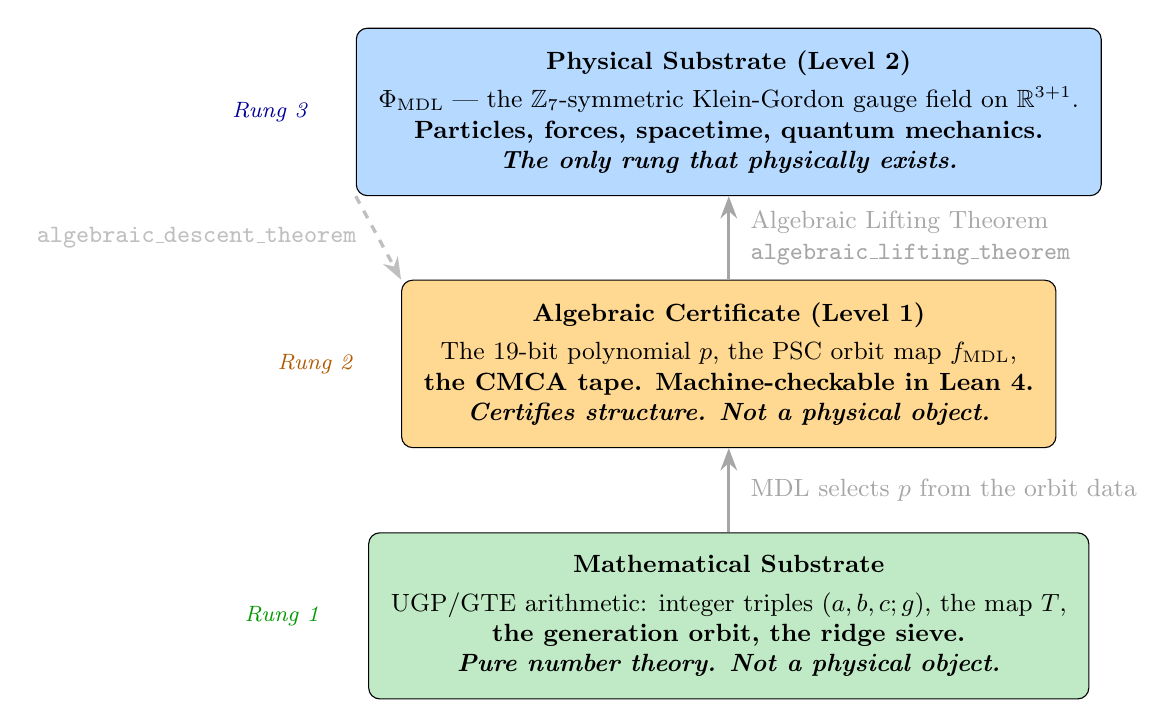
\begin{tikzpicture}[
  rung/.style={draw,rounded corners=4pt,minimum width=8cm,minimum height=1.3cm,
               align=center,font=\bfseries\small,inner sep=8pt},
  arrow/.style={-{Stealth[length=8pt]},very thick,gray!70},
  label/.style={font=\small,align=left},
  every node/.style={font=\small}]

  % Bottom rung: Mathematical Substrate
  \node[rung,fill=runggreen!60,text=black]
    (math) at (0,0)
    {Mathematical Substrate\\[3pt]
     \normalfont UGP/GTE arithmetic: integer triples $(a,b,c;g)$, the map $T$,\\
     the generation orbit, the ridge sieve.\\
     \textit{Pure number theory. Not a physical object.}};

  % Middle rung: Certificate
  \node[rung,fill=rungorange!70,text=black]
    (cert) at (0,3.2)
    {Algebraic Certificate (Level 1)\\[3pt]
     \normalfont The 19-bit polynomial $p$, the PSC orbit map $f_{\rm MDL}$,\\
     the CMCA tape. Machine-checkable in Lean 4.\\
     \textit{Certifies structure. Not a physical object.}};

  % Top rung: Physical Substrate
  \node[rung,fill=rungblue!70,text=black]
    (phys) at (0,6.4)
    {Physical Substrate (Level 2)\\[3pt]
     \normalfont $\PhiMDL$ — the $\ZS$-symmetric Klein-Gordon gauge field on $\mathbb{R}^{3+1}$.\\
     Particles, forces, spacetime, quantum mechanics.\\
     \textit{The only rung that physically exists.}};

  % Arrows up
  \draw[arrow] (math.north) -- node[right=4pt,label]
    {MDL selects $p$ from the orbit data}
    (cert.south);
  \draw[arrow] (cert.north) -- node[right=4pt,label]
    {Algebraic Lifting Theorem\\
     \lean{algebraic\_lifting\_theorem}}
    (phys.south);

  % Down arrows
  \draw[arrow,dashed,gray!50] (phys.south west) -- node[left=4pt,label]
    {\lean{algebraic\_descent\_theorem}}
    (cert.north west);

  % Rung labels on left
  \node[left=0.5cm of math.west,font=\footnotesize\itshape,text=green!60!black]
    {Rung 1};
  \node[left=0.5cm of cert.west,font=\footnotesize\itshape,text=orange!70!black]
    {Rung 2};
  \node[left=0.5cm of phys.west,font=\footnotesize\itshape,text=blue!60!black]
    {Rung 3};

\end{tikzpicture}
\end{center}

\bigskip
\noindent
The three rungs and what lives on each:

\begin{description}[leftmargin=2cm,style=nextline]
  \item[Rung 1 --- Mathematical Substrate]
    The UGP/GTE arithmetic: the ridge sieve, the integer triples $(a,b,c;g)$
    and the map $T$, the generation orbit, and the UWCA evaluator.
    This is pure number theory and combinatorics, prior to any physical
    interpretation.  It is the domain in which MDL's two selections operate:
    the seed selection (the Lepton Seed $(1,73,823)$ from the ridge sieve)
    and the rule selection (the polynomial $p$ from the orbit's parity shadow).
    The mathematical substrate is not a physical object.
    Its role is to \emph{select}: to narrow down, via arithmetic constraints,
    which algebraic certificate is admissible.

  \item[Rung 2 --- Algebraic Certificate]
    What those selections produce: the 19-bit polynomial $p(L,C,R) = C+R-CR-LCR$
    over GF(7), its PSC-orbit map $f_{\rm MDL}$, and the CMCA tape.
    This level enables machine-checkable Lean~4 proofs of algebraic facts ---
    the statements about quantum numbers, generation count, color charges,
    and conservation laws.
    The certificate is not a physical object.
    Its role is to \emph{certify}: to provide machine-checked guarantees about
    what the physical field must contain.

  \item[Rung 3 --- Physical Substrate]
    The continuum field $\PhiMDL$: the $\ZS$-symmetric Klein-Gordon gauge field
    with internal symmetry group $F_{21} = \ZS \rtimes \mathbb{Z}_3$, evolving on
    $\mathbb{R}^{3+1}$.
    This is the only rung that physically \emph{exists}.
    Exact Lorentz invariance, quantum field theory, general relativity, and all
    cosmological observables live at this level.
    Its role is to \emph{be}: to be the actual physical reality.
\end{description}

\begin{tcolorbox}[colback=boxblue,colframe=blue!40!black,
  title=An important clarification]
The word ``substrate'' in this tutorial always refers to the physical substrate ---
Rung~3, $\PhiMDL$.  The word ``mathematical substrate'' (Rung~1) means something
different: the arithmetic ground in which the selection operates.
The mathematical substrate is \emph{not} the physical medium; it is the
mathematical domain of selection.
\end{tcolorbox}

\subsection{The Ladder Is Orthogonal to the ``Levels'' Vocabulary}

The GTE framework also uses a ``level'' vocabulary (Level~0 through Level~3)
to describe the same system at different scales of resolution.
These two vocabulary systems are orthogonal and should not be conflated:

\begin{itemize}
  \item The \term{levels} (0--3) grade the \emph{resolution} at which one physical
    system is described, from the raw polynomial (Level~0) to the continuum
    field (Level~3).
  \item The \term{ladder rungs} name the \emph{roles}: what selects, what
    certifies, what exists.
\end{itemize}

In the levels vocabulary: Levels~0--2 collectively constitute the algebraic
certificate (Rung~2 of the ladder); Level~3 is the physical substrate (Rung~3).
Both vocabulary systems are valid and refer to the same physics; they emphasize
different aspects.

%═════════════════════════════════════════════════════════════════════════════
\section{Why This Is Remarkable}
\label{sec:remarkable}
%═════════════════════════════════════════════════════════════════════════════

\subsection{What Previous CA Proposals Did}

Most CA-based approaches to physics treat the cellular automaton as the physical
substrate itself: the universe is a large grid of discrete cells that update
according to a local rule, and the particles and forces we observe emerge from the
complex collective behavior of this grid.

This approach faces a fundamental obstacle: a finite-resolution grid can never
achieve exact Lorentz invariance.  Various authors have proposed modifications ---
asynchronous updates, random local rules, coarse-graining prescriptions --- but
none resolves the basic tension.

\subsection{What GTE Does Differently}

The GTE framework's contribution is to reposition the cellular automaton:

\begin{tcolorbox}[colback=boxorange,colframe=orange!60!black,
  title=The GTE repositioning]
The CA is a \emph{proof system} for what the continuum field must contain.
It is not the substrate; it is the certificate.
The physical substrate is the continuum field $\PhiMDL$, which has
exact Lorentz invariance.
\end{tcolorbox}

\noindent
This repositioning resolves several long-standing tensions:

\begin{enumerate}[itemsep=6pt]
  \item \textbf{The Lorentz invariance problem is resolved without abandoning CA
    structure.}
    The CA is retained as a proof engine; the continuum field provides exact
    Lorentz invariance.  The no-CA-replica theorem explains why this is the
    only consistent assignment.

  \item \textbf{The zero-free-parameter property becomes possible.}
    If the CA were the substrate, its lattice spacing would be a free parameter.
    Since the CA is a certificate (with no intrinsic spacing), the lattice spacing
    only arises from a calibration reading --- which is derived from the physics,
    not chosen freely.

  \item \textbf{Machine-certified physics becomes achievable.}
    The discrete, finite structure of the CA enables Lean~4 proofs of algebraic
    facts.  The Lifting Theorem ensures these proofs apply to the physical field.
    Over 300 theorems, all zero sorry, connect the 19-bit polynomial to the
    Standard Model.

  \item \textbf{The hierarchy problem is reframed.}
    The enormous ratio between the Planck scale and the hadronic scale
    ($\approx 10^{18}$) is not a mystery requiring explanation by new physics ---
    it is the ratio between two calibrated readings of the same certificate,
    given by GTE arithmetic: $3^{10} \cdot 7^{18}/2^4$.
\end{enumerate}

\subsection{What the Framework Derives, Not Fits}

From the single 19-bit polynomial, with zero free dimensionless parameters
(a single dimensional anchor $m_\tau = 1776.86$\,MeV sets the energy scale):

\begin{center}
\begin{tabular}{@{}ll@{}}
\toprule
\textbf{Derived quantity} & \textbf{Status} \\
\midrule
All 9 charged-fermion masses & $0.295\%$ RMS vs PDG 2022 \\
Electroweak mixing angle ($\sin^2\theta_W$) & zero sorry \\
Strong coupling $\alpha_s(\Lambda_{\rm GTE})$ & CatAD-consistency \\
$\theta_{\rm QCD} = 0$ (strong CP) & 3 independent proofs, zero sorry \\
$\alpha^{-1} \approx 137$ (fine structure) & zero sorry \\
$3+1$ spacetime dimensions & forced, machine-certified \\
Einstein's equations $G_{\mu\nu} = 8\pi G\,T_{\mu\nu}$ & CatAD \\
Newton's constant $G_N$ & $0.040\%$ accuracy \\
Born rule & 4 independent derivations, including CatAL \\
Cosmological constant bracket & enclosing Planck 2018 \\
Baryon asymmetry $\eta_B$ & $+0.15\sigma$ PDG \\
\bottomrule
\end{tabular}
\end{center}

None of these are fitted to data.  They are derived from the structure of the
19-bit polynomial, via the certificate, via the Lifting Theorem, as properties
of the $\PhiMDL$ field.

%═════════════════════════════════════════════════════════════════════════════
\section{Summary}
\label{sec:summary}
%═════════════════════════════════════════════════════════════════════════════

\begin{tcolorbox}[colback=boxblue,colframe=blue!40!black,
  title=The three-sentence summary]
\textbf{The GTE polynomial $p(L,C,R) = C + R - CR - LCR$ over GF(7)} is a 19-bit
algebraic certificate that machine-certifies --- via over 300 zero-sorry Lean~4
theorems --- what structures the physical universe must contain.

\medskip\noindent
\textbf{The physical universe is $\PhiMDL$} --- a $\ZS$-symmetric Klein-Gordon
gauge field on $\mathbb{R}^{3+1}$, whose topological BPS kinks are the elementary
particles of the Standard Model, and whose dynamics generates spacetime, quantum
mechanics, and all cosmological observables.

\medskip\noindent
\textbf{The Algebraic Lifting Theorem} is the certified bridge between the two:
every algebraic fact proved in the discrete CA holds in the continuum field,
and the No-CA-Replica Theorem explains why the continuum field must be
the physical substrate (no finite-resolution CA can achieve exact Lorentz invariance).
\end{tcolorbox}

\bigskip
\noindent
\textbf{The key things to remember:}

\begin{enumerate}[itemsep=8pt]
  \item The CA is the \emph{blueprint}; $\PhiMDL$ is the \emph{building}.

  \item The CA certifies algebraic structure; $\PhiMDL$ provides physical reality.

  \item The No-CA-Replica Theorem is the logical necessity that forces this
    separation: only the continuum field has exact Lorentz invariance.

  \item The Algebraic Lifting Theorem is the bridge: a theorem proved in the CA
    is a theorem about the physical universe.

  \item Particles are BPS topological kinks in $\PhiMDL$, identified by their
    $\ZS$ winding number.  The electron is the $w=4$ kink.

  \item The lattice spacing of the CA has no intrinsic meaning --- it is a
    property of a calibrated reading.  The matter-sector reading gives
    $a \approx 0.097$\,fm (hadronic scale); the Planck reading is a
    working hypothesis.

  \item The ontological ladder has three rungs: mathematical substrate (selects),
    certificate (certifies), physical substrate (exists).  Only the third rung
    physically exists.
\end{enumerate}

\bigskip
\noindent
The full derivation chain is documented across the GTE paper series (P00--P51)
and machine-certified in over 300 Lean~4 modules (zero sorry, zero custom axioms),
all publicly available at \url{https://zenodo.org/records/20560550} and
\url{https://novaspivack.com/research}.



\section*{Further Reading}
\begin{tcolorbox}[colback=orange!8,colframe=orange!50!black,
  title=\textbf{Primary Sources}]
The results in this tutorial are derived in the following papers,
all available open-access on Zenodo and at
\href{https://novaspivack.com/research}{novaspivack.com/research}:
\begin{itemize}
  \item \textbf{P42 --- The $\Phi_{\rm MDL}$ Field} (Lagrangian and kink spectrum):\\
        \href{https://doi.org/10.5281/zenodo.20417576}{doi.org/10.5281/zenodo.20417576}
  \item \textbf{P43 --- The Complete $\Phi_{\rm MDL}$ Framework} (no-CA-replica theorem):\\
        \href{https://doi.org/10.5281/zenodo.20417578}{doi.org/10.5281/zenodo.20417578}
  \item \textbf{P45 --- The Three-Tape CMCA} (3+1D architecture):\\
        \href{https://doi.org/10.5281/zenodo.20465805}{doi.org/10.5281/zenodo.20465805}
  \item \textbf{P48 --- The Complete GTE Framework} (main synthesis monograph):\\
        \href{https://doi.org/10.5281/zenodo.20560550}{doi.org/10.5281/zenodo.20560550}
\end{itemize}
Lean~4 machine proofs: \href{https://github.com/novaspivack/ugp-lean}{github.com/novaspivack/ugp-lean}
\end{tcolorbox}

\bibliography{../../papers/bib/Spivack_Papers_Bibliography}
\end{document}
